% !TEX program = lualatex

\documentclass[12pt]{beamer}
% For handout add ,handout after 11pt

\usetheme{auriga}
\usecolortheme{auriga}

\usepackage{booktabs}
\usepackage{graphicx}
\usepackage[export]{adjustbox}
\usepackage{color}
\usepackage{tikz}

% Set up emoji support with a fallback font
\newfontfamily\emojifont{Apple Color Emoji}[Renderer=Harfbuzz]
\DeclareTextFontCommand{\emoji}{\emojifont}

% Beamer list spacing
% \setlength{\leftmargini}{1.5em}
\setlength{\topsep}{1em}
\setlength{\itemsep}{1em}
\setlength{\parskip}{1.5em}
\setlength{\parsep}{0.5em}

% define some colors for a consistent theme across slides
\definecolor{red}{RGB}{181, 23, 0}
\definecolor{blue}{RGB}{0, 118, 186}
\definecolor{gray}{RGB}{146, 146, 146}
\newcommand{\indep}{\perp\!\!\!\perp}
\title{Above the Line/Below the Line}

\author{Nick Eubank}

\date{\vspace*{.3in} \date}

\newcommand{\empowermenttriangle}[3]{%
    \begin{tikzpicture}[scale=2]
        \draw[thick, black] (0,2) -- (-1.5,0) -- (1.5,0) -- cycle;
        \node[fill=gray!30, rounded corners=10pt, inner sep=8pt, font=\large\bfseries, align=center, text width=4cm] 
            at (0,2.5) {CREATE \\ {\footnotesize #1}};
        \node[fill=gray!30, rounded corners=10pt, inner sep=8pt, font=\large\bfseries, align=center, text width=3.5cm] 
            at (-1.5,-0.6) {COACH \\ {\footnotesize #2}};
        \node[fill=gray!30, rounded corners=10pt, inner sep=8pt, font=\large\bfseries, align=center, text width=4cm] 
            at (1.5,-0.6) {CHALLENGE \\ {\footnotesize #3}};
    \end{tikzpicture}%
}
\newcommand{\dramatriangle}[3]{%
    \begin{tikzpicture}[scale=2]
        \draw[thick, black] (0,2) -- (-1.5,0) -- (1.5,0) -- cycle;
        \node[fill=gray!30, rounded corners=10pt, inner sep=8pt, font=\large\bfseries, align=center, text width=4cm] 
            at (0,2.5) {HERO \\ {\small #1}};
        \node[fill=gray!30, rounded corners=10pt, inner sep=8pt, font=\large\bfseries, align=center, text width=3cm] 
            at (-1.5,-0.6) {VICTIM \\ {\small #2}};
        \node[fill=gray!30, rounded corners=10pt, inner sep=8pt, font=\large\bfseries, align=center, text width=4cm] 
            at (1.5,-0.6) {VILLAIN \\ {\small #3}};
    \end{tikzpicture}%
}

\begin{document}
\setbeamercolor{page number in head/foot}{fg=white}

\begin{frame}[c]{}
    \titlepage
\end{frame}
\begin{frame}
    \frametitle{}
    Moving from teams to self....
\end{frame}

\begin{frame}
    \frametitle{Drama Triangle}
\pause 
    \begin{center}
    \only<2>{\dramatriangle{\phantom{``I'll just do it myself''}}{\phantom{``No one understands''}}{\phantom{``This is your problem. Figure it out''}}}%
    \only<3>{\dramatriangle{``I'll just do it myself''}{\phantom{``No one understands''}}{\phantom{``This is your problem. Figure it out''}}}%
    \only<4>{\dramatriangle{``I'll just do it myself''}{``No one understands''}{\phantom{``This is your problem. Figure it out''}}}%
    \only<5->{\dramatriangle{``I'll just do it myself''}{``No one understands''}{``This is your problem. Figure it out''}}%
    \end{center}
\end{frame}



\begin{frame}
    \frametitle{Empowerment Dynamic}
\pause
    \begin{center}
    \only<2>{\empowermenttriangle{\phantom{Excited by Opportunity}}{\phantom{Suggest Directions}}{\phantom{Believe Can Do Better}}}%
    \only<3>{\empowermenttriangle{Excited by Opportunity}{\phantom{Suggest Directions}}{\phantom{Believe Can Do Better}}}%
    \only<4>{\empowermenttriangle{Excited by Opportunity}{Suggest Directions}{\phantom{Believe Can Do Better}}}%
    \only<5->{\empowermenttriangle{Excited by Opportunity}{Suggest Directions}{Believe Can Do Better}}%
    \end{center}
\end{frame}

\begin{frame}
    \frametitle{Above the Line/Below the Line}

    \begin{center}
    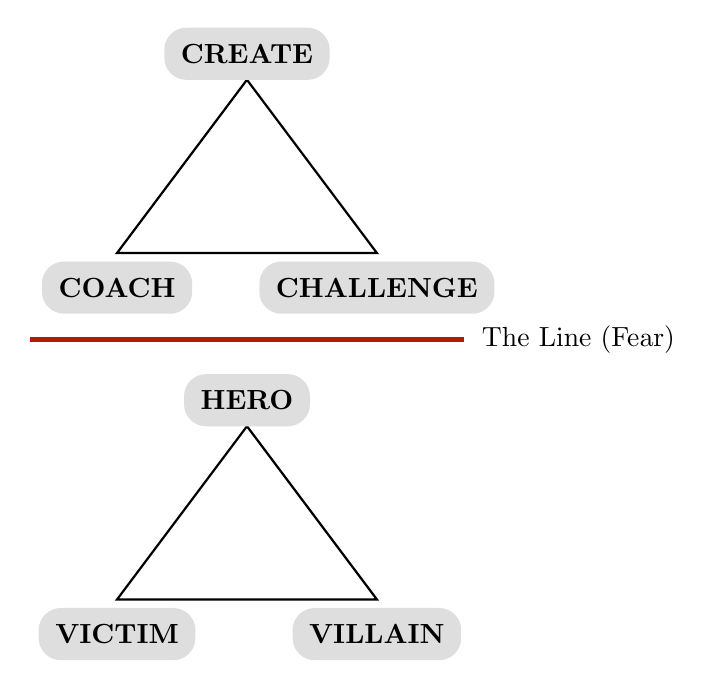
\begin{tikzpicture}[scale=1.1]
        % Shift triangles left
        \begin{scope}[xshift=-1.5cm]
        % Top triangle (CREATE/COACH/CHALLENGE)
        \draw[thick, black] (0,3.5) -- (-1.5,1.5) -- (1.5,1.5) -- cycle;
        
        % Top triangle labels
        \node[fill=gray!30, rounded corners=8pt, inner sep=6pt, font=\normalsize\bfseries] 
            at (0,3.8) {CREATE};
        \node[fill=gray!30, rounded corners=8pt, inner sep=6pt, font=\normalsize\bfseries] 
            at (-1.5,1.1) {COACH};
        \node[fill=gray!30, rounded corners=8pt, inner sep=6pt, font=\normalsize\bfseries] 
            at (1.5,1.1) {CHALLENGE};
        
        % The Line separator
        \draw[line width=2pt, red] (-2.5,0.5) -- (2.5,0.5);
        
        % Bottom triangle (HERO/VICTIM/VILLAIN)
        \draw[thick, black] (0,-0.5) -- (-1.5,-2.5) -- (1.5,-2.5) -- cycle;
        
        % Bottom triangle labels
        \node[fill=gray!30, rounded corners=8pt, inner sep=6pt, font=\normalsize\bfseries] 
            at (0,-0.2) {HERO};
        \node[fill=gray!30, rounded corners=8pt, inner sep=6pt, font=\normalsize\bfseries] 
            at (-1.5,-2.9) {VICTIM};
        \node[fill=gray!30, rounded corners=8pt, inner sep=6pt, font=\normalsize\bfseries] 
            at (1.5,-2.9) {VILLAIN};
        \end{scope}
        
        % The Line label on the right
        \node[font=\normalsize, anchor=west] at (1.1,0.5) {The Line (Fear)};
    \end{tikzpicture}
    \end{center}

\end{frame}

\begin{frame}
    \frametitle{Getting Back Above the Line}
\begin{itemize}
    \item For some people, 10-15 minutes.
    \item Sometimes you need till next day. 
    \item The only antidote to overwhelm is doing nothing.
\end{itemize}
A way to give people space to go from ``Hot Processing'' to ``Cold Processing.''
\end{frame}

\begin{frame}
    \frametitle{Getting Back Above the Line}
The hard part is \alert{noticing when you are below the line}. 
\begin{itemize}
    \item Sometimes you will feel it.
    \item Sometimes you will know you're fearful.
    \item Sometimes you'll find you're \emph{angry} (a friend of fear)
    \item Sometimes you'll notice using Drama Triangle language.
\end{itemize}
\end{frame}


\end{document}
